\textbf{1--3. Fixed-fixed bar.} The schematic identifies the material properties, coordinate, displacement, and two fixed ends.
\begin{figure}[H]
\centering
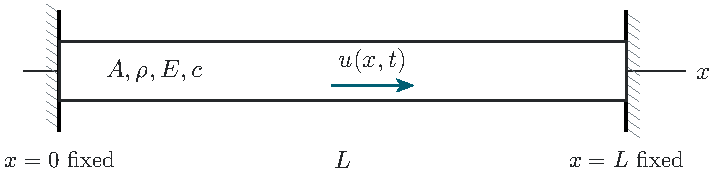
\includegraphics[width=0.78\linewidth]{figures/generated/solutions/C10-bar.pdf}
\caption{Axial vibration of a bar fixed at both ends.}
\end{figure}
The boundary conditions $u(0,t)=u(L,t)=0$ applied to
$U=C_1\sin\gamma x+C_2\cos\gamma x$ give $C_2=0$ and $C_1\sin(\gamma L)=0$. The trivial solution $C_1=0$ yields zero displacement. A nontrivial vibration requires $\sin z=0$, with $z=\gamma L$. Therefore,
\[
z_j=j\pi,\quad \gamma_j=\frac{j\pi}{L},\quad
\omega_j=\frac{j\pi c}{L},\quad f_j=\frac{jc}{2L},\quad
\lambda_j=\frac{2L}{j},\quad L=j\frac{\lambda_j}{2}.
\]
Here $j=1,2,\ldots$, $c=\omega/\gamma$, and $\lambda=2\pi/\gamma$. The first positive frequency is the fundamental, and subsequent modes are overtones. Taking $C_1=1$ gives
\[
\boxed{U_j(x)=\sin\frac{j\pi x}{L},\qquad
\frac{2}{L}\int_0^L U_jU_k\,dx=\delta_{jk},\qquad
\Sigma_j(x)=\frac{Ej\pi}{L}\cos\frac{j\pi x}{L}.}
\]
These conditions and mode forms agree with course-note axial vibration section 3.1, PDF pages 221--225.
